\documentclass{article}
\usepackage[utf8]{inputenc}

\usepackage{amsthm}
\usepackage{amsfonts}
\usepackage{amsmath}
\usepackage{amssymb}
\usepackage{fullpage}
\usepackage{graphicx}
\usepackage[usenames]{color}
\usepackage{hyperref}
  \hypersetup{
    colorlinks = true,
    urlcolor = blue,       % color of external links using \href
    linkcolor= blue,       % color of internal links 
    citecolor= blue,       % color of links to bibliography
    filecolor= blue,        % color of file links
    }
    
\usepackage{listings}
\usepackage{textgreek} % added so I could add the epsilon in text
\usepackage{tipa} % added so I could add the pipe symbol |

\definecolor{dkgreen}{rgb}{0,0.6,0}
\definecolor{gray}{rgb}{0.5,0.5,0.5}
\definecolor{mauve}{rgb}{0.58,0,0.82}

\lstset{frame=tb,
  language=haskell,
  aboveskip=3mm,
  belowskip=3mm,
  showstringspaces=false,
  columns=flexible,
  basicstyle={\small\ttfamily},
  numbers=none,
  numberstyle=\tiny\color{gray},
  keywordstyle=\color{blue},
  commentstyle=\color{dkgreen},
  stringstyle=\color{mauve},
  breaklines=true,
  breakatwhitespace=true,
  tabsize=3
}

\theoremstyle{theorem} 
   \newtheorem{theorem}{Theorem}[section]
   \newtheorem{corollary}[theorem]{Corollary}
   \newtheorem{lemma}[theorem]{Lemma}
   \newtheorem{proposition}[theorem]{Proposition}
\theoremstyle{definition}
   \newtheorem{definition}[theorem]{Definition}
   \newtheorem{example}[theorem]{Example}
\theoremstyle{remark}    
  \newtheorem{remark}[theorem]{Remark}


\title{CPSC-402 Report}
\author{Stephen White}

\date{\today}

\begin{document}

\maketitle

\begin{abstract}
In short, the goal is to search for all occurrences of a small string within a larger string. We are trying to emulate the text searching abilities of Regular Expressions. 
\end{abstract}

\tableofcontents

\section{Introduction}\label{intro}

My name is Stephen White. I am a Computer Science major with a minor in Business Administration at Chapman University.

\section{Homework}\label{homework}

This section contains the solutions to the homework. 

\subsection{Week 1}

%For most weeks, you will have a subsection that contains your answers.

\subsubsection{Homework 1.1}
The homework discussed in this section can be seen \href{https://hackmd.io/@alexhkurz/rycnvMvgu}{here}.
Part 1 of the homework is exercise 2.2.4 item B. The problem can be found on page 54 of the textbook (page 69 of the pdf).
\newline \newline
The first question is as follows: "Give DFA's accepting the following languages over the alphabet \{0,1\}: The set of all strings with three consecutive 0's (not necessarily at the end)."
\newline\newline
My answer to this question is as follows:\\
Since we know that this DFA's alphabet can only consist of 0's and 1's, and we are searching for three consecutive 0's, looking like this: 000, we can formally defined the DFA as 
\begin{align*}
    \{\omega\ |\ \omega\ is\ of\ the\ form\ x000y\ for\ some\ strings\ x\ and\ y\ consisting\ of\ 0's\ and\ 1's\ only \}
\end{align*}

The following image is a diagram of this DFA showing its states and transitions.\\
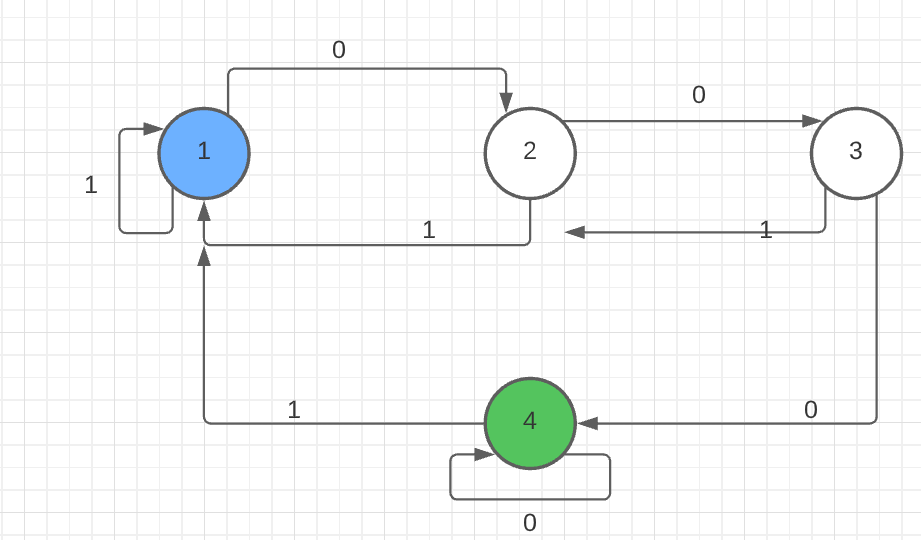
\includegraphics{Question224PartB.png}\\
(I have chosen blue to signify the initial state and green to signify the success state)\\

The next question asks "Give DFA's accepting the following languages over the alphabet \{0,1\}: The set of strings with 011 as a substring."\\\\
My answer to this question is as follows:\\
Since we know that this DFA's alphabet can only consist of 0's and 1's, and we are searching for the string 011, we can formally defined the DFA as 
\begin{align*}
    \{\omega\ |\ \omega\ is\ of\ the\ form\ x011y\ for\ some\ strings\ x\ and\ y\ consisting\ of\ 0's\ and\ 1's\ only \}
\end{align*}

The following image is a diagram of this DFA showing its states and transitions.\\
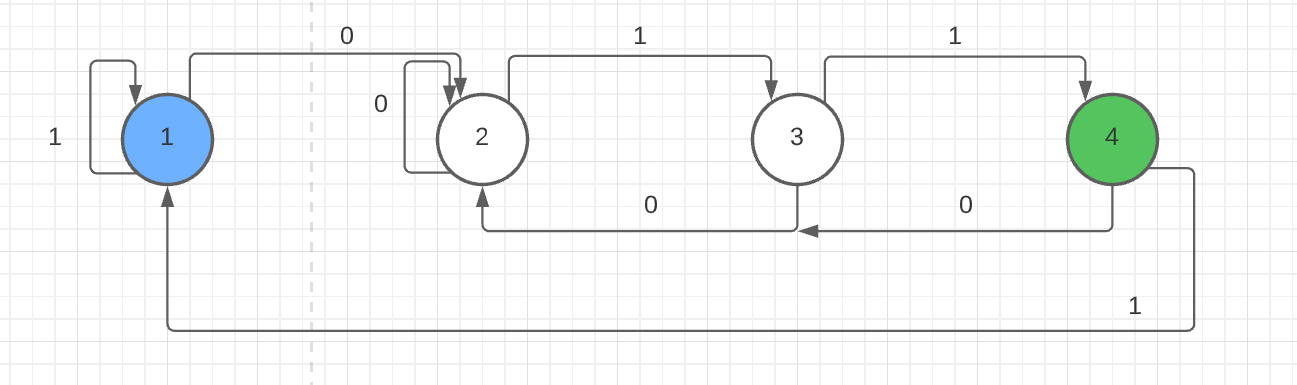
\includegraphics[scale=0.75]{Question224PartC.png}\\
(I have chosen blue to signify the initial state and green to signify the success state)\\

\subsubsection{Homework 1.2}
The homework discussed in this section can be seen \href{https://github.com/alexhkurz/compiler-construction-2022/blob/main/homework-1.2.md}{here}.\\\\

Part 1 of this assignment is to answer the following question: 
\begin{center}
    "Does the file contain the sequence aa or abb? For example, if the file is aaabbaabb, the output should be [2,3,5,7,9]. The challenge here is to not write a program that runs twice through the file, once to search for aa and once for abb, but to find a way of running through the file only once and to simultaneously search for both strings."
\end{center}

I chose to write the program in C\# because I am most familiar with it, and I believe it has a good mix between control and programming speed. That code can be found \href{https://github.com/mamba72/CompilerConstruction_Assignments/blob/main/Reports/ReportResources/StringSearchingImplementation.cs}{here on my GitHub}.
To aid me in my understanding of the problem, I made the following diagram of the DFA I was creating:\\
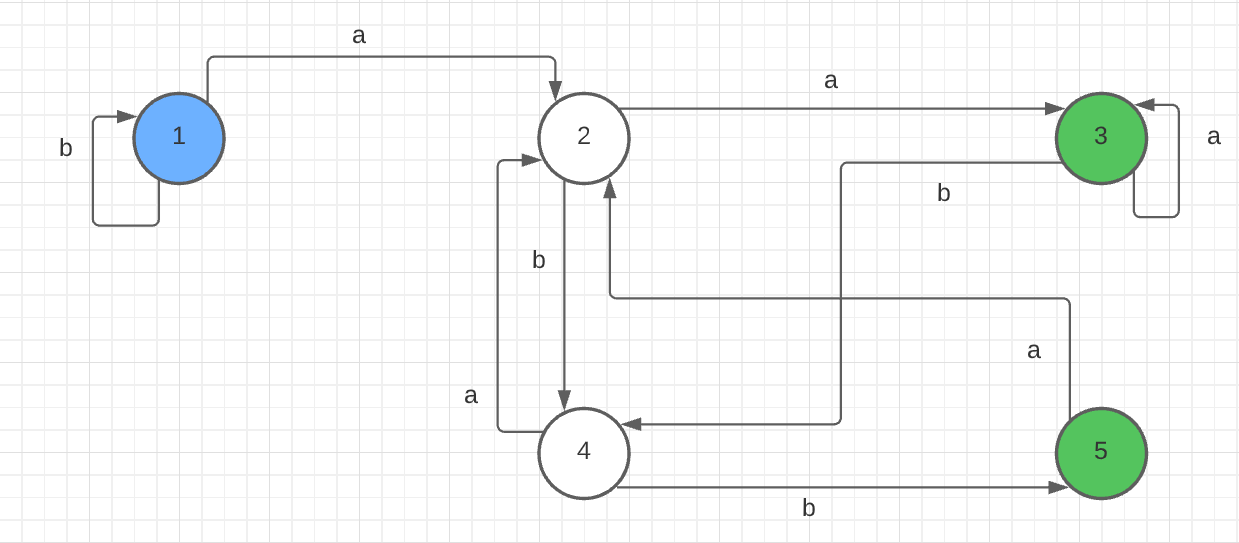
\includegraphics[scale = 0.7]{Question3DFA.png}\\\\

Part 2 of the homework was to complete exercise 2.2.10 (the proof being optional) on page 54 of the textbook (page 70 of the pdf).\\
The question reads as follows:
\begin{center}
    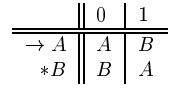
\includegraphics[]{Exercise2210Diagram.png}\\
"Informally describe the language accepted by this DFA."
\end{center}
I tackled this problem by first breaking down the chart, to understand what I was being asked. The chart is similar to a Punnett Square. The left column is a list of the possible current states (an input). The top row is a list of possible character inputs. The rest of the chart is the next state (the output) determined by that row's current state and current character. Since the only possible characters are 1 and 0, the language accepted by this DFA is a set of strings or words created by any combination of 0's and 1's. 


\subsection{Week 2}

\subsubsection{Homework 2.1.1 Composing Automata}
The homework discussed in this section can be found \href{https://hackmd.io/@alexhkurz/ryV_FU7XI}{here}.\\
\textbf{Exercise 2.3.4}\\
Part 1 of this assignment is to answer the following questions:\\
\\
Find NFAs that recognize:\\
\includegraphics[scale=0.3]{Questions 2-3-4.png}\\

\textbf{Part A:}\\
The NFA I created is outlined in the diagram below.
\begin{center}
    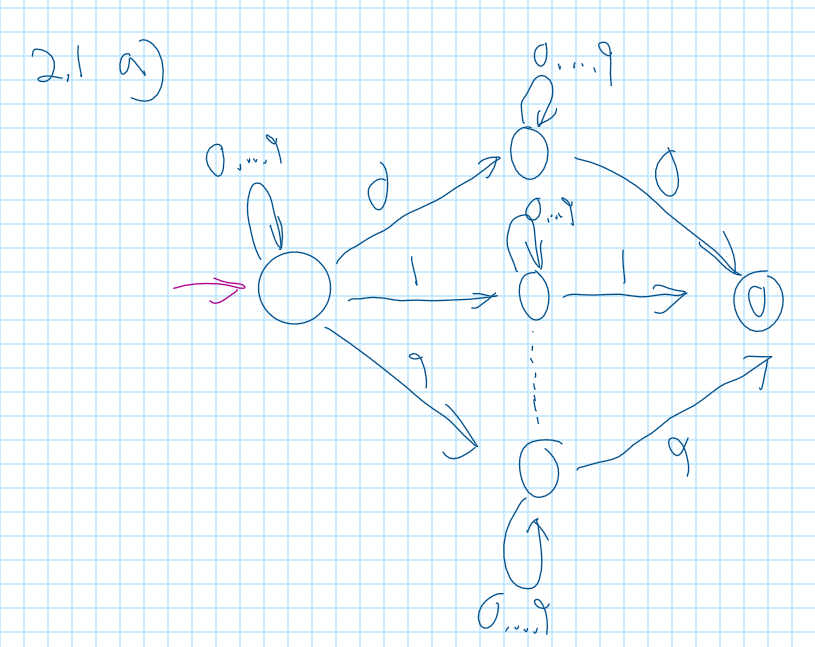
\includegraphics[scale=0.5]{Diagram 2-1-1a.png}
\end{center}
I used the "..." as a way to simplify the diagram and make it more readable by not writing every state, but enough to understand the diagram. 
The idea of the NFA is to ensure that the only way to reach the success state is to have crossed over the last digit before. 
The most helpful part for my understanding was to look at the transition to the success state has the same condition as the transition to the mid-state. 
This ensures that the digit has been seen before in the string.\\
\\
\textbf{Part B:}\\
The NFA I created is outlined in the diagram below.
\begin{center}
    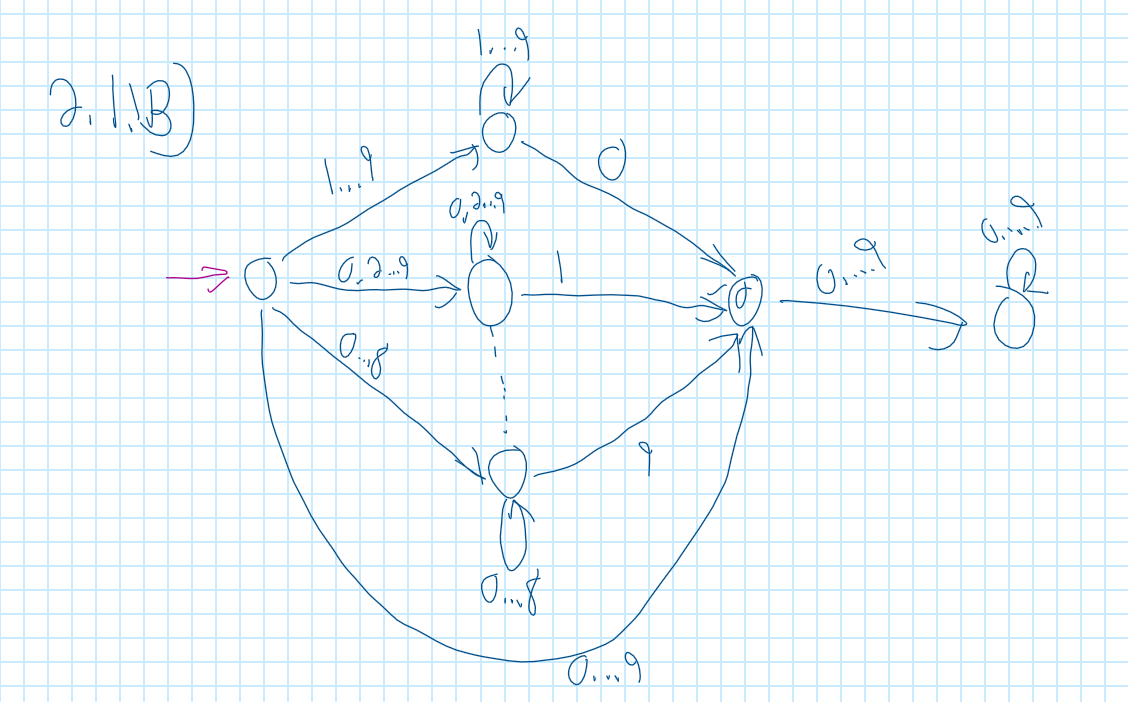
\includegraphics[scale=0.45]{Diagram 2-1-1b.png}
\end{center}
The main idea of this NFA is to ensure that the only way to reach the success state is to have never seen the last digit before in the string.
The part that helped me understand this NFA the most is knowing that it is effectively the complement of part A. 
So to accomplish this, I used the same foundation as the one from part A, but the transitions from the initial state are all digits except the one I'm looking for. For example, the top path is only successful if the final digit is zero, so the first transition includes all numbers 1 through 9, to prevent the possibility of 0 being seen elsewhere in the string. In addition to this, I added another state after the success to prevent the success state from firing if the transition is taken before the end of the string.\\
\\
\textbf{Part C:}\\
The NFA I created is outlined in the diagram below.
\begin{center}
    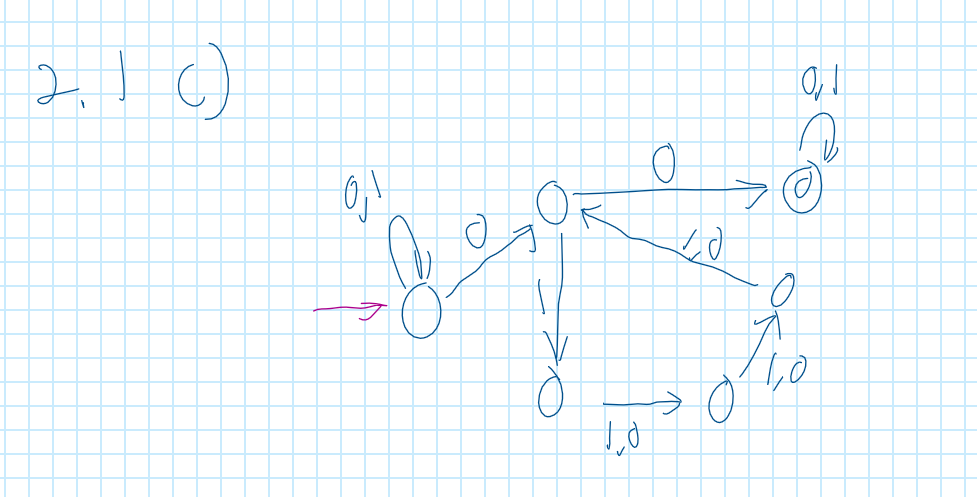
\includegraphics[scale=0.5]{Diagram 2-1-1c.png}
\end{center}
The main challenge with this problem is to count multiples of 4, including 0. 
I tackled this challenge by having 3 states with 4 transitions that effectively "count" the digits between 0's.
Since the problem states that the entire string doesn't have to be encased by the 0's, I have loops on the initial and success states that enable the NFA to count an entire word that contains the 0's.\\
\\
\textbf{Exercise 2.5.3}\\
Part 2 of this assignment is to answer the following questions:\\
\\
Find \textepsilon-NFAs that recognize:\\
\includegraphics[scale=0.6]{Questions 2-5-3.png}\\
\\
\textbf{Part A:}\\
The NFA that I created is outlined in the diagram below.
\begin{center}
    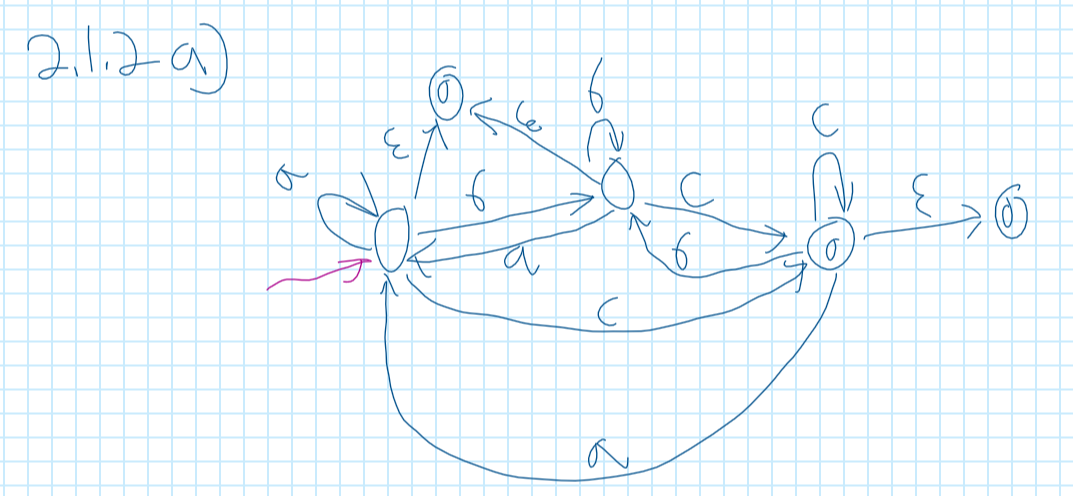
\includegraphics[scale=0.5]{Diagram 2-1-2a.png}
\end{center}
The main challenge with this NFA is the fact that there can be zero of each character. This diagram gets complex very quickly because we are looking for a pattern of alphabetical strings, but there is no guarantee that it will contain an 'a', 'b', or 'c'.
While solving this problem, there was some confusion around the phrase "consisting of." I chose to take that similar to "having substrings of" rather than "being entirely made of." If it meant "a string entirely made of a's, b's, and c's in alphabetical order", then the diagram would be slightly different and less complex.\\

\textbf{Part B:}\\
The NFA that I created is outlined in the diagram below.
\begin{center}
    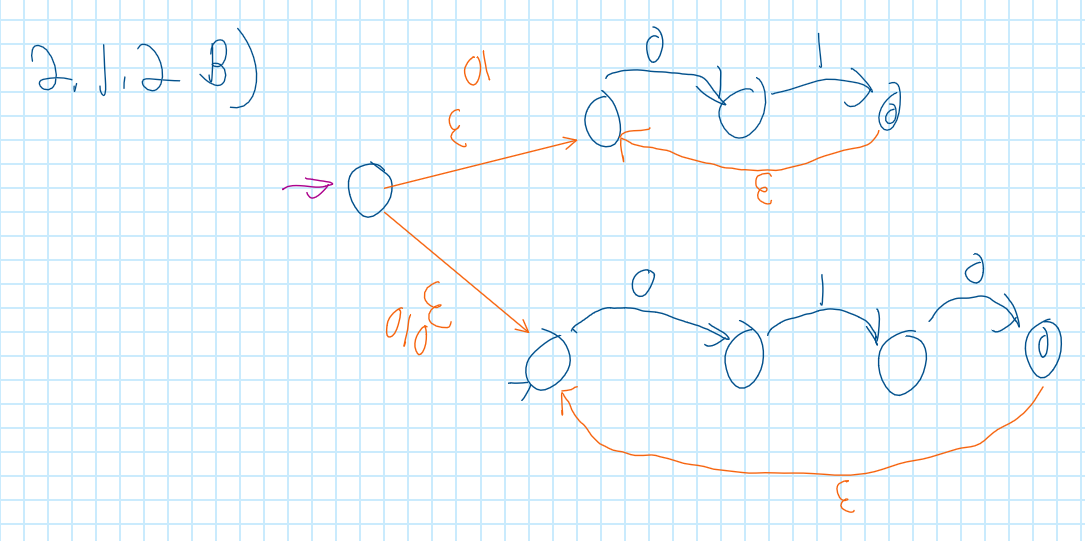
\includegraphics[scale = 0.5]{Diagram 2-1-2b.png}
\end{center}
This problem had "composition" written all over it. From the start, I noticed that this would be two automata working in parallel. 
The top section is what identifies the "01" repeating pattern while the bottom section identifies the "010" pattern. 
To "join" these two sections, I performed epsilon jumps to the beginning of each section immediately from the initial state.
To simplify the possibility of a repeating pattern, I simply jump from the success states back to that section's starting state.\\

\textbf{Part C:}\\
The NFA that I created is outlined in the diagram below.
\begin{center}
    \includegraphics[scale = 0.5]{Diagram 2-1-2c.png}
\end{center}
The main challenge with this problem was figuring out how to count 10 positions from the last. If I were implementing this program, I would simply iterate from the back of the string rather than the start, but we are unable to do that with our current setup. 
To overcome this, I created a loop of both 0's and 1's on the initial state to allow for strings longer than 10.
I then have 9 states (10 transitions) that upon finding a 1, enter the success state. If one of those states finds a 0, it will simply move onto the next position.\\

\subsubsection{Homework 2.2.1 Regular Expressions}
The homework discussed in this section can be found \href{https://hackmd.io/@alexhkurz/S1EVYe7bO}{here}.\\
This homework was to write regular expressions for the languages in exercises 2.3.4 and 2.5.3 (the problems from the previous homework).\\
\textbf{Exercise 2.3.4}\\
\textbf{Part A:}
The regular expression for part A of exercise 2.3.4 is as follows:
\begin{center}
    \textit{( 0 + ... 9) * ( 0 ( 0 + ... 9 ) * 0 + ... )}
\end{center}
(We had gone over this in class.) The "..." is used to simplify and shorten the writing of the expression rather than writing all the digits 0 through 9.

\textbf{Part B:}
The regular expression for part B of exercise 2.3.4 is as follows:
\begin{center}
    \textit{( 1 + ... 9 ) * 0  + ( 0 + 2 + ...9 ) * 1 + ( 0 + 1 + 3 + ...9 ) * 2 + .... (0 + ...8 ) * 9 + \textepsilon }
\end{center}
This regular expression gets all the strings where the last digit has no appeared before in the string.

\textbf{Part C:}
\begin{equation}
    (0+1)^*\ 0\ ((0+1)^4)^*\ 0\ (0+1)^*
\end{equation}
For this problem, I needed some help. I utilized the website \href{https://regex101.com/}{Regex101} to help me create this regular expression. Since the above expression is not directly applicable in most programming languages, the regular expression I came up with in Regex is this:" \textit{.* 0 ((0\textpipe1)\{4\})* 0 .*} ".

\textbf{Exercise 2.5.3}\\
\textbf{Part A:}\\
The regular expression for part A is as follows:
\begin{center}
   \textit{a* b* c*}
\end{center}
This was was very simple because the * is what allows the preceding character to appear anywhere between 0 and unlimited number of times.\\

\textbf{Part B:}\\
The regular expression for part B is as follows:
\begin{center}
    \textit{(01)(01)* + (010)(010)*}
\end{center}
For this problem, I needed some help again. The regular expression I came up with in Regex101 is this: \textit{(01)(01)+\ \textpipe\ (010)(010)+}\\

\textbf{Part C:}\\
The regular expression for part C is as follows:
\begin{equation}
    (0+1)^* 1 (0+1)^n\ ,\ where\ 0 <= n <= 9
\end{equation}

Since this question says that the number 1 must appear in the last 10 digits and we have the ability to use exponents in our definition, I'm using N as a way to ensure that the 1 can show up anywhere in the last 10 positions. I also had some help from \href{https://regex101.com/}{Regex101} for this problem and the equivalent expression I got in Regex101 while I was working on this problem was " \textit{.* 1 (1\textpipe0)\{0,9\}\$} ".

\subsection{Week 3}
\subsubsection{Homework 3.1 Converting NFAs to DFAs}
The homework discussed in this section can be found \href{https://hackmd.io/@alexhkurz/HylLKujCP}{here}.\\
\textbf{Exercise 2.3.1}\\
Part 1 of this assignment is to answer the following question:
\begin{center}
    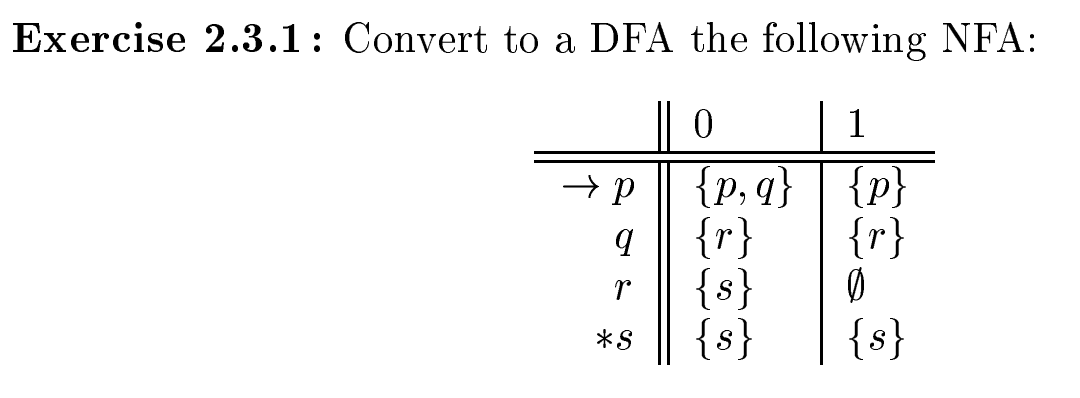
\includegraphics[scale=0.25]{Question231Chart.png}
\end{center}

The diagram for the DFA can be found below:
\begin{center}
    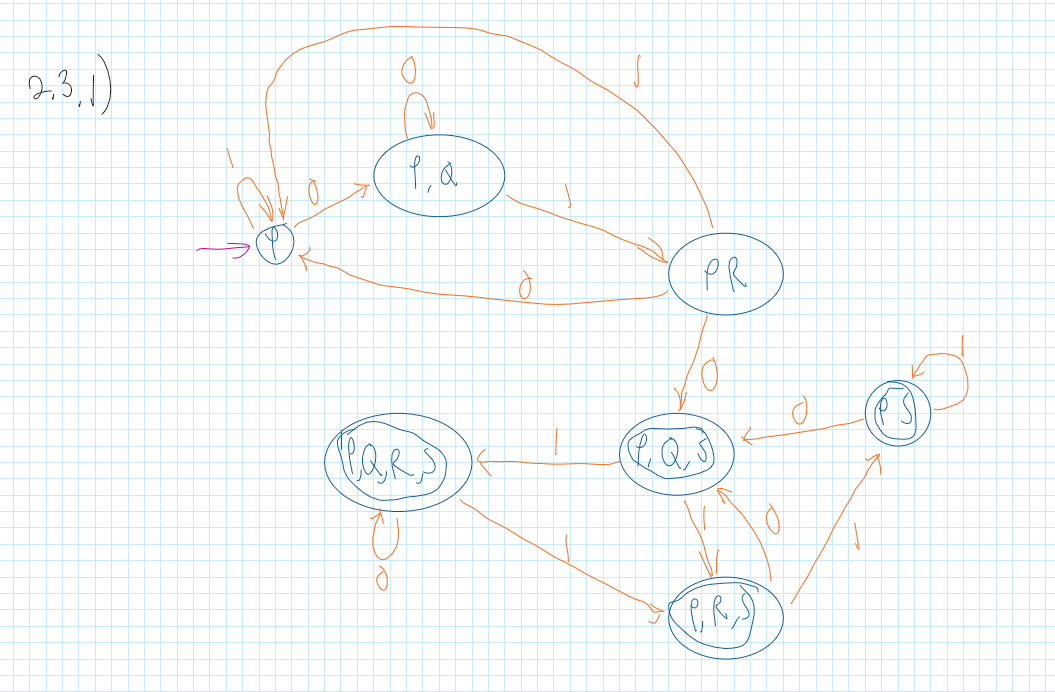
\includegraphics[scale=0.55]{Diagram 2-3-1 DFA.png}
\end{center}
\\
\textbf{Exercise 2.3.2}
Part 2 of this assignment is to answer the following question:
\begin{center}
    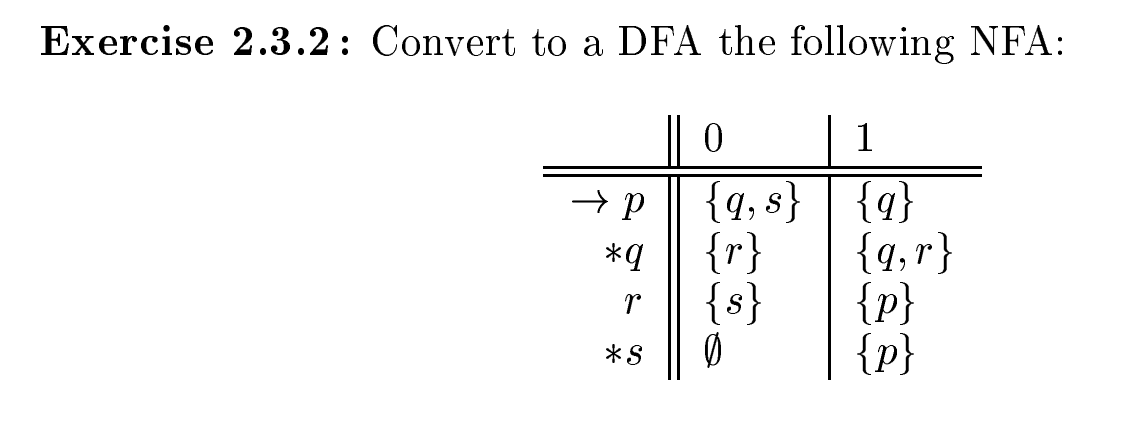
\includegraphics[scale=0.25]{Question232Chart.png}
\end{center}

The diagram for the DFA can be found below:
\begin{center}
    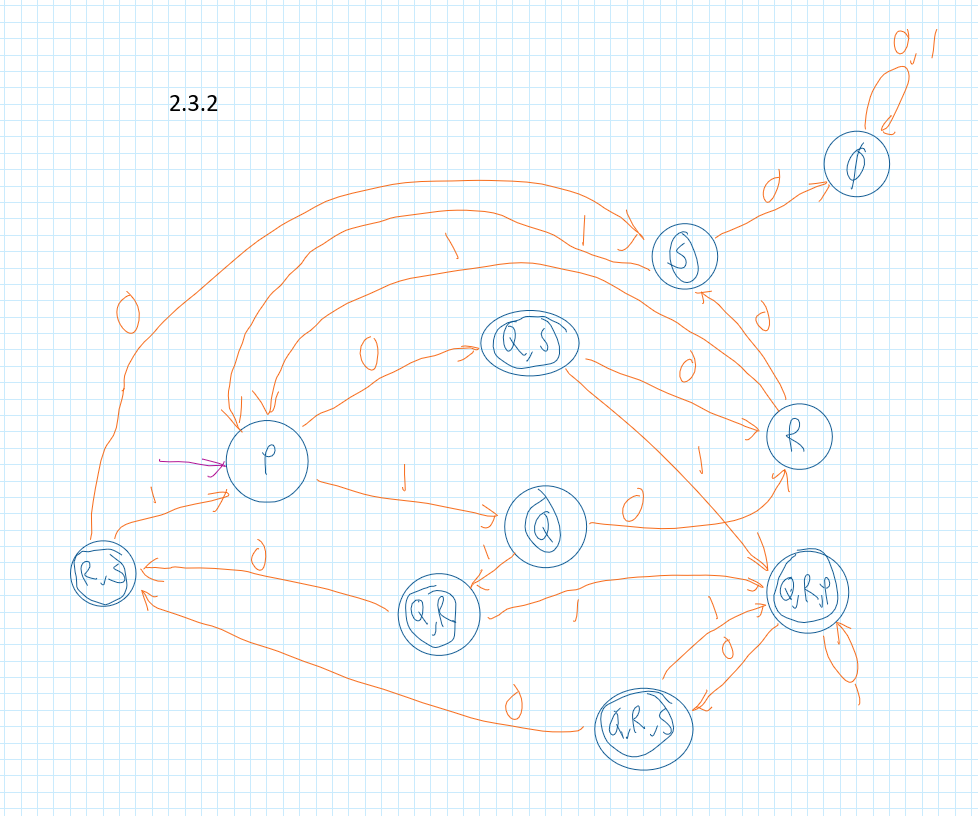
\includegraphics[scale=0.5]{Diagram 2-3-2 DFA.png}
\end{center}
\\
\textbf{Exercise Converting NFAs to DFAs in Haskell}

Part 2 of this assignment is to complete the following task:
\begin{center}
"Put the definitions of dfa\_initial, dfa\_final, dfa\_delta in the report and explain your code in a paragraph. Also put your modified version of automata05.hs in your github repository.)

The file automata05 provides a template, in which you have to modify lines 71, 72, 73. Complete the definition of nfa2dfa as described in the three bullet points above and test it with various examples."
\end{center}

My code can be seen below:

\begin{lstlisting}[language=Haskell]
-- convert an NFA to a DFA
nfa2dfa :: NFA s -> DFA [s]
nfa2dfa nfa = DFA {
  -- exercise: correct the next three definitions 
  dfa_initial = [nfa_initial nfa],
  --dfa_final = let final qs = True in final,
  dfa_final = 
   let 
    --final var1 var2 = (var1 var2)
    --final nfa = disjunction nfa
    --final 
    --final [s] = disjunction(nfa_final s)
        --final (q:qs) = final qs
      --final var1 = (final (nfa_final var1))
      --final qs = [nfa]
      final qs = map (disjunction) (qs)
      


   in final,
  dfa_delta = 
   let 
    delta qs c = qs 
    --delta [] c = 
    --delta (q:qs) c = 
   in delta }
\end{lstlisting}

Sadly, I was unable to complete this section. I am confident in my answer for dfa\_initial, but I'm far from confident for dfa\_final and dfa\_delta. 
I tried to comment all of my attempts in order to show the many thought processes I had. 
I also hope that one of them was close. I think the hardest part for me was understanding the data types of all of the variables and knowing what was being passed into the function in the first place. 
I was really struggling with understanding how to use what felt like Object Oriented Programming inside of a functional language. 

\section{Project}

The project will be to compile code from a programming language of your choice to assembly and to explain the assembly code and compilation process using the knowledge your learned in this course. 


\medskip\noindent
Pro tips:
\begin{itemize}
\item Choose a compiled (not interpreted) programming language.
\item Choose a language that you find interesting anyway.
\item Start early.
\item Come to office hours. I have not run this part of the course before and I am really interested what you will find.
\end{itemize}
 
\section{Conclusions}\label{conclusions}

%(approx 400 words)

%In the conclusion, I want a critical reflection on the content of the course. Step back from the technical details. How does the course fit into the wider world of programming languages and software engineering?

\begin{thebibliography}{99}
\bibitem[HMU]{Hopcroft}
	John E. Hopcroft, Rajeev Motwani, Jeffrey D. Ullman:
\href{http://ce.sharif.edu/courses/94-95/1/ce414-2/resources/root/Text%20Books/Automata/John%20E.%20Hopcroft,%20Rajeev%20Motwani,%20Jeffrey%20D.%20Ullman-Introduction%20to%20Automata%20Theory,%20Languages,%20and%20Computations-Prentice%20Hall%20(2006).pdf}{Introduction to automata theory, languages, and computation,} 3rd Edition. Pearson international edition, Addison-Wesley 2007

\end{thebibliography}

\end{document}
